\chapter{考察}
\label{chapter:consideration}
本章では, 実験環境に関する考察, 提案手法に関する考察および実環境への適用を考えた時の課題を考察する. 

\section{提案手法についての考察}
本節では, 提案手法のパラメータに関してどのように挙動が変化するのかを示し, どのようにパラメータを背絵亭するべきなのかについて議論する. 

\subsection{リンクコストパラメータに関する考察}
前述の評価実験において, リンクコストベースの経路切替手法が経路状況に対応し, 経路が切り替わるタイミングが変化することによって,
デッドラインベースの単純な経路切替手法における問題を解消することを示した. 
式(\ref{linkcost})に示すリンクコストは, 大きく二つの項から構成されている. 
一つは$\alpha \cdot \nu(t)^\beta$であり, 経路状況によって変化する項である. 
もう一方は, $\gamma (t - t_{deadline})^\delta$であり, デッドライン時間に関する項である. 
それぞれの項にはパラメータ$t_{deadline}, \alpha \sim \delta$があり, 今回の評価実験では,
それぞれ$t_{deadline}=300[ms]$, $\alpha=1, \beta=1, \gamma=1, \delta=1$と設定した. 
しかし, 二つの項の変数を考えると, それぞれのパラメータによって経路が切り替わるタイミングが変動する. 

今, リンクコストベースの切替手法における各パラメータ毎の挙動の違いを評価する.  
この評価ではエンドノード間の1対1の通信を想定しており, ベンチマークトラフィックには, iperfを用いて継続してデータ転送を行った.  
また, トポロジーとしてk=4 DHFTを用いる. 
このトポロジーでは, エンドノード間の等価な通信経路が2つあり, それぞれSLとLLに割り当てている. 
そしてそれぞれのレーンに対し通信負荷を与えることで経路の状況を変化させる. 
SLに対する通信負荷には, 64KBのフローを200msに1回ポアソン生起するトラフィックを用いる. 
LLに対する通信負荷には, 実験時間中継続してデータ転送を行うトラフィックを用いる. 
それぞれの通信負荷については, Senderノードの数を変化させ, 負荷の度合いに対する評価を行う. 
なお, パラメータ$t_{deadline}$は$300[ms]$を設定している. 

経路状況に対する挙動に関わるパラメータ$\alpha,
\beta$を変化させたときの経路切替時間の移り変わりをFig.\ref{fig:basic_para_link}に示し, 横軸はSL, LLへの通信負荷の強度を表すSenderノードの数, 縦軸には通信が発生したときの時間を0としたときの経路切替時間を示している. 
この結果から, パラメータ$\alpha$が大きくなればなるほど, 経路状況の変化にアグレッシブに反応し, また値が小さいと
パラメータ$t_{deadline}$の影響を大きく受けることとなり, 設計目的の期待の狙い通りの結果が得られた. 
実際, SLでのSenderノードが増えれば増えるほど, SLでのキューイング遅延が大きくなり, SLのリンクコストの値が大きくなる. 
これは, SLで通信をするよりもLLで通信を行ったほうが有利であると判断された結果であり, このため切替時間が短くなる. 
また, LLでのSenderノードが増えれば増えるほど, LLでのキューイング遅延が大きくなり, LLのリンクコストが大きくなる. 
これは, LLへ切り替えて通信するよりもSLに留まって通信を継続した方が有利であると判断された結果であり, このため切替時間が長くなる. 

\begin{figure}[t]
    \begin{center}
    \includegraphics[autoebb, width=250pt]{./img/param_alpha.pdf}
    \caption{Basic performance path switching based on
    link-cost according each parameter $\alpha$}
    %\ecaption{The control loop in DCTCP}
    \label{fig:basic_para_link}
    \end{center}
\end{figure}


次にデッドラインに対する挙動に関わるパラメータ$\gamma,
\delta$を変化させたときの経路切替時間の移り変わりをFig.\ref{fig:basic_para_dead}に示す.
この結果から, パラメータ$\gamma$が大きくなればなるほど, 経路状況よりも$t_{deadline}$に大きく依存することとなり,
設計の狙い通りの結果が得られた.
実際, LLでのSenderノードが増えれば増えるほど, LLでのキューイング遅延が大きくなり, SLに留まるような判断がされるが,
$t_{deadline}$を超えれば経路切替が発生しやすくなるような挙動をする.
そのため, 切替時間が$t_{deadline}$を大きく超えるような挙動は発生しない. 

\begin{figure}[t]
    \begin{center}
    \includegraphics[autoebb, width=250pt]{./img/param_gamma.pdf}
    \caption{Basic performance path switching based on
    link-cost according each parameter $\gamma$}
    \label{fig:basic_para_dead}
    \end{center}
\end{figure}

今回の評価の際にはべき乗部分にあたる$\beta, \delta$については固定して評価を行った. 
これはリンクコスト計算においてべき乗の影響は大きく, 一方を大きくするとその項が支配的に作用するためである. 
リンクコストの定義の意味を考慮して, $\beta=\delta$と設定し, それぞれの項の次元をを揃えることが望ましいと考える. 

$t_{deadline}$については, 対象となるアプリケーションが最低限満たすべき通信時間の値を設定するべきである. 
一般に, 近年のデータセンターにおける並列分散処理アプリケーションでは, 300ms以内に通信を終えるべき\cite{key-value2}であるとしており,
評価実験においてもその値に従った.

$\alpha, \gamma$については, 通信状況に対し機敏に反応させたければ, $\alpha$を大きく, $\gamma$を小さく設定するべきである. 
しかし, それらを極端な値に設定すると, 一方のレーンに通信が偏る可能性がある. 
また, しきい値を満たすショートフローの割合を大きくするには, $t_{deadline}$を本来のしきい値より小さくし, $gamma$を大きく,
$\alpha$を小さくすれば良い. 
これにより, SLへの負荷を減らすことができ, SLを良好な状態に保つことができ,
アプリケーション要求を満たすフローの割合を大きくすることができると考えられる. 
ネットワーク環境に最適なパラメータについては, そのネットワークが持つレーン数や, アプリケーションによって決まると考えられる. 

\section{実験環境についての考察}
本節では, データセンタレーンモデルを利用した実験環境に関して, レーン構成の違いとそれを実現するためのトポロジーについて考察する. 

\subsection{データセンタレーンモデルに対する考察}
レーンの割り当て方には様々な組み合わせが考えられる. 
今回の評価実験では, 基本的にエンドノード間の物理的に異なる経路が二つあることを想定し, それぞれに対しSL, LLを割り当てた. 
今後, MPTCPが普及していくと, 今以上にエンドノードにおいて複数のインタフェースを持つことが考えられる. 
実際, エンドノードが複数NICを持ち, マルチホーミングな通信を実現することは, エンドノードのネットワーク処理改善の解決方法の一つと考えられる. 
その時, 異なる物理パスがインタフェースの数だけ用意することが可能となる. 
$\S$\ref{sec:throughput}の基本性能に関する評価実験では, 3つの経路がある環境において, 1つをSLに割り当て,
残りをLLに割り当て, 経路切替を行った. 
この構成では, 経路が切り替わる前は最大一経路分, 切り替わった後には最大二経路分のスループットを達成できる. 

3つの経路がある環境では, 2つをSLに割り当て, 残りをLLに割り当てる構成が考えられる. 
この時の時系列ごとのスループットの変化をFig.\ref{fig:basic_comparison_sl2_ll1}示す.
評価環境は, $\S$\ref{sec:throughput}と同様である. 
SLが2経路あるため, 通信開始当初は, 2経路分の通信性能を出すためにウィンドウサイズを増加させていく. 
リンクコストベースの切替手法では, 増加の過程で切替が生じ, LL1経路分の通信性能へ収束する. 
デッドラインベースの切替手法では, デッドライン時間を迎えるまでに最大帯域利用可能となり, 経路切替まで2経路分の通信性能を実現できている. 
これはSLに1経路しか割り当てられていない場合に発生していた通信開始直後の遅延問題を解消できる可能性がある. 
実際, MPTCPで用いられている輻輳制御には, より有利な経路に対しウィンドウサイズを拡大していくというアルゴリズムがあるので,
混雑した経路の影響を抑えることができると考える. 
しかし, 切替が生じた場合, 1経路分の性能しか出せないのでMPTCPによる効果が現れない. 

また, 4つの経路がある環境において, 2経路ずつそれぞれSL, LL二割り当て流構成も考えられる. 
この時の時系列ごとのスループットの変化をFig.\ref{fig:basic_comparison_4path}示す.
評価環境は, $\S$\ref{sec:throughput}と同様である. 
SLが2経路あるため, 通信開始当初は, 2経路分の通信性能を出すためにウィンドウサイズを増加させていく. 
そして経路切替により, LL2経路分の通信性能を実現できている. 

このように, 異なる経路(エンドノードにおけるそれぞれのインターフェース)によって, SLとLLの組み合わせを変更することができる. 
しかし, LLの性質から考えると, 長い時間, 大きなサイズの通信を行うフローが最終的に切り替わって来るため, より大きなスループットを出すためにも,
LLになるべく多く経路を割り当てるように設定する必要がある. 

\begin{figure}[t]
    \begin{center}
    \includegraphics[autoebb, width=250pt]{./img/sl2_ll1.pdf}
    \caption{Basic performance comparisons with 2 SLs and a LL}
    \label{fig:basic_comparison_sl2_ll1}
    \end{center}
\end{figure}

\begin{figure}[t]
    \begin{center}
    \includegraphics[autoebb, width=250pt]{./img/4path.pdf}
    \caption{Basic performance comparisons with 4paths}
    \label{fig:basic_comparison_4path}
    \end{center}
\end{figure}

\subsection{MPTCPを有効活用するトポロジーに関する考察}

ネットワーク帯域の効率的な利用を目指す取り組みとして, 様々なデータセンターネットワークトポロジーが提案されている. 
提案されているトポロジーは, 複数の等コストな経路がある冗長性を持たせた構成になっており, そうした経路を有効活用する手段としてMPTCPがある. 
$\S$\ref{sec:traffic}に示したように, MPTCPを用いることで,
将来の広帯域化により発生すると予想されているノード側のボトルネックについても, 解決することができると期待されており,
デュアルホーミングを活用したトポロジーも提案されている\cite{improving}. 
具体的には, 今日のサーバでは一般的である複数のNICに対してMPTCPを利用するということである. 
そこでエンドノードの持つ複数のNICを有効活用するためのトポロジーの一つの提案として, マルチホーミングなFatTree(Multi-Homing
FatTree)が考えられる.  

Fig.\ref{fig:multi-homing}にk-MHFTを示す. 
k-aryマルチホーミングトポロジーはFatTreeと同様に, k個のポッドから構成されおり, 
一つのポッドで$k/2, k^2/4$それぞれaggregatorスイッチとedgeスイッチを持つ. 
aggregatorスイッチとedgeスイッチではそれぞれ,
$k/2$のノードと上位レイヤーのスイッチ1つに接続し, 計$k/2+1$ポートが必要である. 
また, coreスイッチは$k/2$台の$k/2$ポートスイッチが必要である. 
さらに, MHFTは$k^3/4$までのノードを持つことができ, $k/2$のインタフェースが必要であるとする. 
この時, $k/2$本の経路が, 物理的に等価なコストの経路数となる. 
このトポロジーによって, 多様なデータセンター内でのトラフィックに対し, 複数のレーンから構成されるデータセンターレーンモデルにおいて,
通信負荷分散することが可能となる.

しかし, 今日の巨大なクラスターを持つデータセンターの設計には, 性能の優位さだけではなく構築に掛かるコストについても考慮しなければならない. 
そこで, MHFT構築に掛かるコストについて, 保有できるエンドノードの台数とともに検討を行う. 
検討には, エッジ部分でのスイッチとして48ポート1ギガビットスイッチ(\$7000)とアグリゲーション,
コア部分でのスイッチとして128ポート10ギガビットスイッチを用いて構成する際のコストを検討する\cite{fattree}.
なお, 配線ケーブルのコストは考慮しないこととする. 

Fig.\ref{fig:MHFT_cost}に, 保有できるホストの数とトポロジー形成に掛かる費用の関係を示す. 
例えば, 20000ホストに対するスイッチ機器を考えたとき, Fattreeトポロジーでは, 1152台のedgeスイッチ,
1152台のAggregationスイッチ, 576台のcoreスイッチによって構成することができ, かかる費用は約\$1217Mである. 
一方MHFTにおいて20000ホストを保有するトポロジーを構築しようとすると,  27648台のedgeスイッチ,
1152台のAggregationスイッチ, 24台のcoreスイッチによって構成することができ, かかる費用は約\$1016Mである. 

このように, MHFTではコスト面では有効であると言える.
しかし, FatTreeに比べ, 等コストな経路の数は少なくなっており, 通信負荷分散の可能性としてはFatTreeの方が潜在している.

\begin{figure}[t]
    \begin{center}
    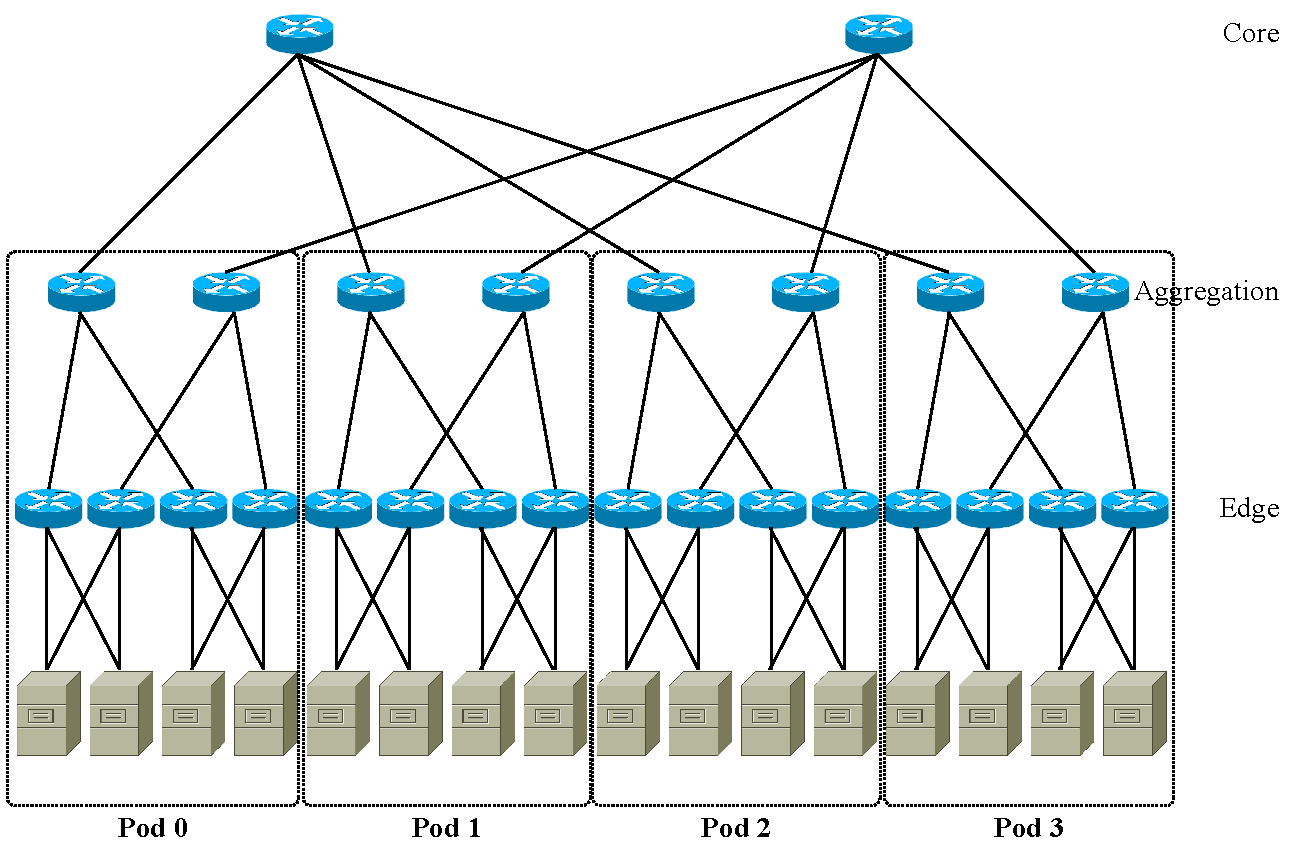
\includegraphics[autoebb, width=250pt]{./img/mhft.pdf}
    \caption{k=4 Multi-homing in the FatTree Topology}
    %\ecaption{The control loop in DCTCP}
    \label{fig:multi-homing}
    \end{center}
\end{figure}

\begin{table}[t]
    \begin{center}
    \caption{Multi-homing FatTree constitution}
    \begin{tabular}{c|c|c}
    k-ary & Number & Port/Interface \\ \hline
    core & $k/2$ & $k/2$ \\ \hline
    aggregator & $k^2/2$ & $k / 2 + 1$ \\ \hline
    edge & $k^3 / 4$ & $k / 2 + 1$ \\ \hline
    node & $k^3 / 4$ & $k / 2$ \\
    \hline
    \end{tabular}
    \label{table:mhft_constitution}
    \end{center}
\end{table}


\begin{figure}[t]
    \begin{center}
    \includegraphics[autoebb, width=250pt]{./img/mhft_cost.pdf}
    \caption{Current cost estimation vs. maximum possible number of hosts}
    %\ecaption{The control loop in DCTCP}
    \label{fig:MHFT_cost}
    \end{center}
\end{figure}

\section{実環境への適用に関する考察}
本節では, 実環境への提案手法の実装についての課題を考察する. 

\subsection{MPTCPアドレスペアの問題に関する考察}
現状のMPTCPの実装上, サブフローを形成する際での信負荷の分散が有効に働かない問題がある. 
今, Fig.\ref{fig:mptcp_pair}のような複数インタフェースを持つエンドノード間の通信を考える. 
この時, 現状のMPTCP実装では, 互いのアドレスを交換(ADD\_ADDRESS)しあった後,
フルメッシュな組み合わせのIPアドレスでサブフローが形成される. 
具体的には, 1つのTCPコネクション(F1{src:10.1.0.1, dst:10.2.0.1})と3つのサブフロー(F2{src:10.1.0.1,
dst:10.2.1.1}, F3{src:10.1.1.1, dst:10.2.0.1}, F4{src:10.1.1.1,
dst:10.2.1.1})が形成される. 
静的なIPベースのルーティングを想定した環境において, フローF1はサーバ側へのデータパケット通信に対してData:S1-S2-S4,
クライアント側へのACKパケット通信に対してはACK:S1-S2-S4の経路をそれぞれ用いる. 
同様に, フローF2はData:S1-S2-S4, ACK:S1-S3-S4, フローF3は, Data:S1-S3-S4,
ACK:S1-S2-S4, フローF4は, Data:S1-S3-S4, ACK:S1-S3-S4の経路をそれぞれ通る. 
基本的にデータパケット通信の方がデータサイズもパケットの数も多いため, キューイング遅延がより起こりやすい通信であり, 例えばフローF1と
F2では異なるサブフローにも関わらず, Dataパケットは同一の経路を通る. 
また, MPTCPはそれぞれのフローを同一のものとして輻輳制御を行うため, 経路によってはトラフィックが偏る可能性があり, 有効的な経路利用を実現できない. 

今回のような複数の経路を持つネットワーク環境において, 通信不可の分散の点から理想的なサブフローの形成は,
1つのTCPコネクション({src:10.1.0.1, dst:10.2.0.1})と1つのサブフロー({src:10.1.1.1,
dst:10.2.1.1})が形成されることである. 
すなわち, 1インタフェース1サブフローの原則による, 重複のないIPアドレスのペアを形成することで, 最適なトラフィック負荷の分散を実現できる. 
そのため, 本提案手法の実装にあたり, 既存のMPTCP実装に対して変更が必要であった. 

\begin{figure}[t]
    \begin{center}
    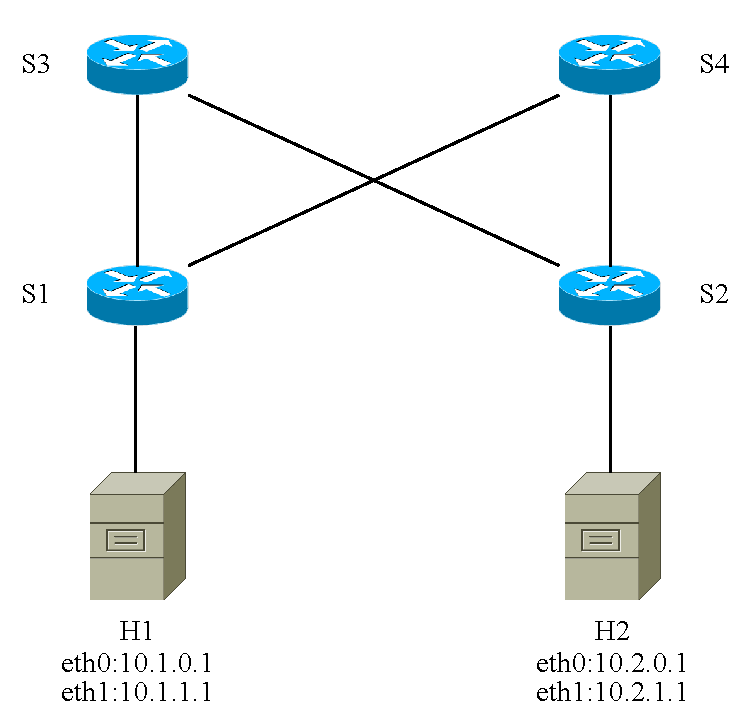
\includegraphics[autoebb, width=250pt]{./img/pair_problem.pdf}
    \caption{Techinical problem of creating subflow without complete paired IP
    addressses}
    %\ecaption{The control loop in DCTCP}
    \label{fig:mptcp_pair}
    \end{center}
\end{figure}

\section{今後の課題について}
本節では, データセンターが抱える性能障害の問題に対し, 提案手法が今後どのような解決策を提示できるのかについての考察と,
実環境における適用の際の課題について考察する. 

\subsection{Incast問題に対する考察}
データセンターが抱える性能障害の一つにIncast問題がある\cite{incast}. 
これは, 一つのインタフェースに大量のショートフローが同時に集中することにより遅延が生じるという, データセンターでの並列分散処理が生み出す特有の問題である. 
今回の提案手法では, Queue buildupに対するアプローチであるために, このIncast問題に対して有効に働く手立てはない. 
しかし, データセンターレーンモデルによる通信の切り分けによって, この問題を解決できる可能性がある. 
今のMPTCP実装では, サイズの小さい通信には複数経路を用いずに一つの経路だけで通信が完了するため, 今回の提案手法のような経路切替手法は有効に働かない.
そのため, 今回のような複数経路への負荷分散を考えた場合, あらかじめ通信する経路を分散させる必要がある. 
このような静的な負荷分散として, ラウンドロビンやハッシュベースを用いた負荷分散手法がある.
しかし, これらの手法ではその不完全な負荷分散によって,
Fig.\ref{repflow_scenario}のようにロングフローとショートフローが同じ経路を使って通信する場合がある. 
今回提案したデータセンターレーンモデルはではそれらのフロー区別して制御することができ, SLを利用するショートフローに対してのみ,
負荷分散の効果を与えることができる. 
例えば, エンドノード間の通信経路が3本存在している時には, SLに2経路, LLに1経路割り当てた時, 
SLに対してラウンドロビンやハッシュベースを用いた負荷分散手法が有効であると考える.
そこで, 3経路のうち, SLに2経路, LLに1経路割り当てた時のIncastトラフィックに対する負荷分散の予備実験を行った. 
検証環境は, Fig.\ref{fig:lane_model}のようなSLがに2経路割り当てられているトポロジーを考える. 
このトポロジーでは, 左右に20ノードずつ計40ノードが接続されている. 
ベンチマークトラフィックとして, 70KBフローに対し平均200msのポアソン生起を行う. 
通信を行うノードの数の割合を大きくしていき, incastトラフィックによる通信負荷を大きくする. 
この時, ラウンドロビンによる負荷分散と一つの経路を占有する状況を比較する. 
Fig.\ref{fig:robin}に結果を示す. 
縦軸がincastトラフィックに対する平均FCT, 横軸は通信ノードの割合を示している. 
この結果はラウンドロビンが理想的に働いた時の結果を意味しているが, 提案したデータセンターレーンモデルでは, こうした同地に扱って良いフローに対してのみ,
負荷分散を適用することができるため, その効果は大きいと考えられる. 

\begin{figure}[t]
    \begin{center}
    \includegraphics[autoebb, width=250pt]{./img/robin.pdf}
    \caption{Effect of the load balancing by simple idea with Round-Robin
    alghorithm}
    %\ecaption{The control loop in DCTCP}
    \label{fig:robin}
    \end{center}
\end{figure}

\subsection{実環境における適用, 運用に関する考察}
本提案手法では, 各ノードが複数のインターフェースがあり,
等価なコストの経路がインタフェース数だけ用意されているマルチパスなネットワーク環境での利用を想定しており,
エンドノードOSの変更のみで実環境への適用が可能となる.
この時, 各インタフェースに割り当てられているIPアドレスが独立して通信を行えるようなルーティング設定が必要となる. 
今回の評価実験では, ルーティングについては各スイッチでのスタティックルーティングにより環境を構築した. 

今日の大規模データセンターにおいては, 機器の故障やメンテナンス等で, 一部のリンクがダウンすることは比較的頻繁に起こり\cite{trouble},
常に完全対称なトポロジーの運用は困難である.
特に本提案手法では, 宛先IPアドレスによる経路負荷分散がなされている事が前提であるために, 局所的に通信ができない部分があると,
提案手法による効果が小さくなる.
今回の実装では, そういった一部の経路が利用できなくなった際のフォールバックMPTCPによる複数経路利用に一任するという点で課題がある. 
実際, ネットワーク障害の度に, 適切なルーティングを考慮し, マニュアルでルーティングとエンドノードOSへ設定の修正を加えるのは現実的ではない. 
こういった運用の課題については近年,  OpenFlowという技術によって,
ネットワークの柔軟な制御を実現することが可能となってきており, 今後の活用が期待されている\cite{openflow}.
現時点ではデータセンター内のネットワーク機器でOpenFlowに対応している機器は少ないが, 今後, こういった小規模な障害, トラブルの対応に対し,
運用面での活用できる可能性をを秘めている. 

 
